\documentclass[a4paper, 11pt]{article}
\usepackage[utf8]{inputenc}

\usepackage[french]{babel}
\usepackage{graphicx} 
\usepackage{hyperref}
\usepackage{xcolor}
\usepackage{listings}
\usepackage{enumitem}
\usepackage{amsmath} 
\usepackage{amsfonts}
\usepackage{hyperref}
\usepackage{array,booktabs,makecell,multirow}
\usepackage{siunitx}
\usepackage[left=2cm, right=2cm, bottom=2cm, top=2cm]{geometry}
\usepackage{algorithm}
\usepackage{algorithmic}
\usepackage{minted}
\RecustomVerbatimEnvironment{Verbatim}{BVerbatim}{}
\newcommand{\HRule}{\rule{\linewidth}{0.5mm}}

\begin{document}

\begin{titlepage}

\begin{center}

\includegraphics[scale = 0.35]{logo.jpg}\\
\vspace{1cm}
\textsc{\huge Université de Liège}\\[1.2cm]
\HRule \\[1cm]
\textsc{\LARGE Programmation fonctionnelle (INFO0054-1) }\\[1cm]
{\Huge \bfseries Projet : Tableaux Sémantiques}\\[1.4cm] 
\HRule \\[1cm]
\end{center}

\begin{minipage}{0.45\linewidth}
      \begin{flushleft} \large
        \emph{Authors : } \\
        Louis \textsc{Hogge}  s192814\\
        Merlin \textsc{Michel}  s193209\\
        Tom \textsc{Weber}  s203806
      \end{flushleft}
\end{minipage}
\hfill
\begin{minipage}{0.45\linewidth}
      \begin{flushright} \large
        \emph{Professor : } C. \textsc{Debruyne}\\
        \emph{Year : } 2022-2023 
      \end{flushright}
\end{minipage}

\end{titlepage}

\newpage

\section{Proposez}
\subsection{Des règles d’élimination pour EQUIV, XOR, NAND,
et XNOR.}

\begin{figure}[!h]
    \centering
    \begin{subfigure}[a]
        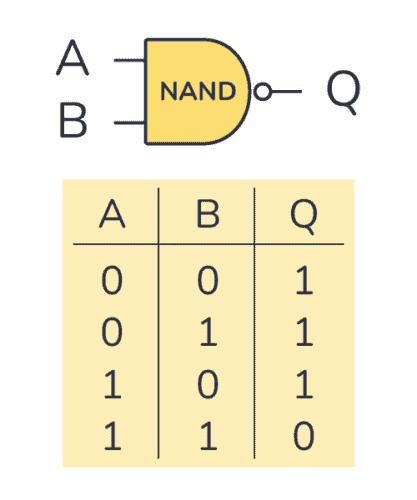
\includegraphics[width=0.2\linewidth]{NAND.png}
        \label{NAND}
    \end{subfigure}
    \begin{subfigure}[b]
        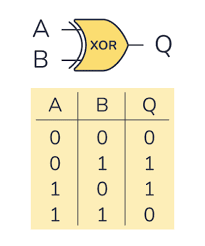
\includegraphics[width=0.2\linewidth]{XOR.png}
        \label{XOR}
    \end{subfigure}
    \begin{subfigure}[c]
        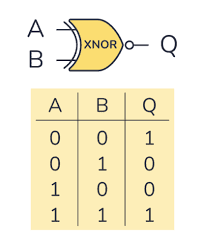
\includegraphics[width=0.2\linewidth]{XNOR.png}
        \label{XNOR}
    \end{subfigure}
\end{figure}

En se basant sur les tables de vérité ci-dessus, nous pouvons déduire les règles d'élimination suivantes :\\
\begin{math}
\begin{array}{l}
\{\neg(A \wedge B)\} \Rightarrow\{\neg A\},\{\neg B\} \\
\{(A \oplus B)\} \Rightarrow\{A, \neg B\},\{\neg A, B\} \\
\{(A \odot B)\} \Rightarrow\{A, B\},\{\neg A, \neg B\}
\end{array}
\end{math}\\
pour NAND, XOR et XNOR respectivement.\\
Nous avons également remarqué que EQUIV pouvait s'écrire \\
\begin{math}
\{A \leftrightarrow B\} \Rightarrow\{(A \rightarrow B ) \wedge(B \rightarrow A)\}
\end{math}\\
ce qui nous donne exactement les mêmes résultats que pour XNOR en suivant les règles d'élimination implémentées précédemment.

\subsection{Une extension pour les opérateurs OR et AND
prenant n $\neq$ 1 arguments.}
Afin de généraliser les formules OR et AND pour un nombre d'argument $ n \geq 1 $, nous devons nous mettre d'accord sur le comportement de ces formules en fonction de leur nombre d'arguments.\\
Tout d'abord, pour OR, nous avons élargi le concept précédemment utilisé afin d'affirmer que la formule était vraie si \textbf{au moins} un parmi ses arguments d'entrée est vrai.\\
Ensuite, nous avons fait de même pour AND stipulant que pour que la formule soit vraie, il fallait que touts les arguments d'entrée soient vrais.
\begin{figure}[!h]
    \centering
    \begin{subfigure}[a]
        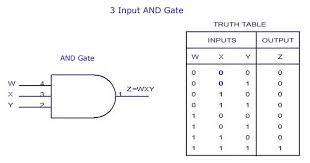
\includegraphics[width=0.4\linewidth]{AND3.jpg}
        \label{AND3}
    \end{subfigure}
    \begin{subfigure}[b]
        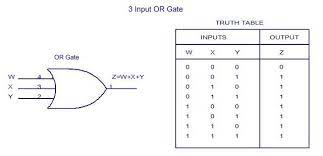
\includegraphics[width=0.4\linewidth]{OR3.jpg}
        \label{OR3}
    \end{subfigure}
\end{figure}


\section{Décrivez la représentation que vous avez utilisée pour
les formules et les tableaux.}
\subsection{Formules:}
Pour représenter les formules nous avons décidé d'opter pour une  \textit{sealed abstract class} supérieure représentant l'entité "Formule de Logique Propositionnelle":\\

\begin{figure}[htp]
    \centering
    \begin{minted}{scala}
    sealed abstract class PLF
  \end{minted}
\end{figure}\\

où PLF signifie \textbf{P}ropositional \textbf{L}ogic \textbf{F}ormula. Le mot-clef \textit{sealed} restreint l'endroit où nous pouvons définir les sous-classes, cela doit être fait dans le même fichier source. Le mot-clef \textit{abstract} empêche la création d'objet à partir de la classe \textit{PLF}, oblige à passer par les classes qui étendent cette \textit{sealed abstract class} supérieure et permet à cette-dernière de faire office d'unique parent (les classes qui étendent \textit{PLF} ne peuvent hériter d'aucune autre \textit{abstract class}).\\

Ce choix nous permet d'étendre cette classe avec l'ensemble de nos formules définies sous la forme de \textit{case class}:\\

\begin{figure}[htp]
    \centering
    \begin{minted}{scala}
    case class AF(s : String) extends PLF 
    case class AND(lf : PLF*) extends PLF
    case class OR(lf : PLF*) extends PLF
    case class IFTHEN(f1 : PLF, f2 : PLF) extends PLF
    case class NOT(f1 : PLF) extends PLF
    case class NAND(f1 : PLF, f2 : PLF) extends PLF
    case class XOR(f1 : PLF, f2 : PLF) extends PLF
    case class XNOR(f1 : PLF, f2 : PLF) extends PLF
    case class EQUIV(f1 : PLF, f2 : PLF) extends PLF
  \end{minted}
\end{figure}\\

 L'utilisation de \textit{case class} permet de bénéficier des avantages suivant:
 \begin{itemize}
     \item Une liste de paramètres unique qui sert également de constructeur
     \item Pas besoin du mot clef \textit{new}
     \item Tous les paramètres sont immuables et publiques
     \item Les instances sont comparées par structure et non par référence
 \end{itemize}
\textcolor{white}{blankline}\\

 Une autre possibilité aurait été d'utiliser un \textit{enum} mais le premier avantage concernant la liste de paramètres unique servant également de constructeur nous a semblé le plus compétitif.
 

\subsection{Tableaux:}
Pour représenter les tableaux nous avons fait le choix de travailler avec des \textit{List} afin de pouvoir bénéficier de l'ensemble des méthodes qu'offre cet objet disponible par défaut dans les librairies Scala. Ces méthodes pré-implémentées représentent un avantage considérable et évitent de devoir réinventer la roue. Les \textit{List} sont, en outre, tout à fait adaptées à la résolution du problème proposé, cela grâce à leur capacité de regrouper des éléments communs et, par conséquent, de les différencier d'autres collections d'éléments.\\

Une autre possibilité aurait pu être d'implémenter un nouvel ADT \textit{Tree} afin de s'approcher le plus possible de la représentation que l'on a du problème. Cependant, comme précisé, l'arbre n'est qu'une vue de l'esprit et implémenter l'ADT \textit{Tree} ne représente pas un avantage comparé aux \textit{List} et leurs méthodes associées pré-implémentées dans les librairies Scala.

\section{Décrivez vos choix d'implémentation pour les règles
d'élimination.}
Afin d'implémenter les règles d’élimination nous avons créer la fonction suivante:
\begin{figure}[htp]
    \centering
    \begin{minted}{scala}
    def eliminationRule(f: PLF): List[List[PLF]] = f match
        case ...
        ...
    \end{minted}
\end{figure}
 se basant sur un pattern matching permettant d'obtenir un code concis et lisible tout en offrant la possibilité de faire correspondre les \textit{PLF} à des patterns de formules de logique propositionnelle. Ces patterns correspondent donc aux règles alpha et bêta données dans l'énoncé du projet ainsi qu'aux extensions de la partie 3. Chaque \textit{case} renvoie ainsi les outputs souhaités sous la forme de \textit{List}, commune pour les règles alpha (formules conjonctives) et différentes pour les règles bêta (formules disjonctives).

\section{Décrivez vos choix d’implémentation pour l’extension.}
Tout d'abord, pour les différentes extensions, nous avons fait le choix d'utiliser le caractère * afin afin de définir un "varargs field" pour un argument d'entrée sous forme d'une séquence.\\
Pour le AND, il nous a suffit de créer une liste contenant tous les arguments à l'aide de la fonction toList().\\
Pour le OR, il nous a fallut parcourir chaque argument de manière récursive afin de créer une liste pour chacun d'entre eux.

\section{Décrivez l’utilisation de vos modules et donnez des
exemples.}

\begin{itemize}
\item
On represente nos atomics avec AF("string") et NOT(AF("string")).
Ensuite on peut joindre ces atomics avec des formules logiques. 
Ex: IFTHEN(AF("q") , NOT(AF("r"))) 

\item
Pour construire des set de formules, il suffit de placer ces dernières dans un List().

\item
Utilisation des différentes fonctions:

Dans la fonction main(), creer un "val" = l'ensemble de formule qu'on veut tester.
Je mets un exemple de chaque fonction mais bien on peut bien sûr utiliser les fonctions sur les autres list de formules.

\item
Pour ce qui est des extansions (EQUIV, XOR, NAND, XNOR), ils marchent de la même manière que les autres formules.
Et avec OR et AND prenant n $\geq$ 1 arguments, il suffit d'enchainer les atomics à l'intérieur. Ex: OR(AF("p"), AF("q"), AF("r"))

\end{itemize}
\begin{minted}{scala}
def main(args : Array[String]): Unit = 
    import PLF._

    // une List() avec une seule formule
    val plf1 = List(IFTHEN(AF("p"), IFTHEN(AF("q"), AF("r"))))

    // une List() avec un set de 2 formules
    val plf2 = List(
                    IFTHEN(AF("p"), IFTHEN(AF("q"), AF("r"))), 
                    NOT(IFTHEN(IFTHEN(AF("p"), AF("q")), AF("r")))
                    )
    
    // une List() avec un set de 3 formules
    val plf3 = List(
                    IFTHEN(AF("p"), IFTHEN(AF("q"), AF("r"))), 
                    NOT(IFTHEN(IFTHEN(AF("p"), AF("q")), AF("r"))), 
                    OR(AF("p"), AF("q"), AF("r"))
                    )

    semtab(plf3)

    isSatisfiable(plf3)

    isValid(List(AND(AF("p"), AF("q"))), (AF("q")))

    isTautology(OR(AF("p"), NOT(AF("p"))))

    isContradiction(AND(AF("p"), NOT(AF("p"))))

    models(List(OR(AND(AF("q"), AF("p")), AND(AF("r"), AF("p")))))

    counterexamples(List(AF("c"), AF("d"), OR(AF("a"), AF("b"))), AF("a"))
\end{minted}

\section{Sources images}
\begin{itemize}
    \item Øyvind Nydal Dahl, "Logic Gates",  //www.build-electronic-circuits.com/category/logic-gates/, 15 septembre 2022 (\ref{NAND}).
    \item john, "What are Digita", Logic Gates and their types?", //www.circuitstoday.com/logic-gates, 27 février 2021 (\ref{AND3}).
\end{itemize}

\end{document}